\documentclass[letterpaper]{article}
\usepackage{amssymb}
\usepackage{fullpage}
\usepackage{amsmath}
\usepackage{epsfig,float,alltt,epstopdf}
\usepackage{psfrag,xr}
\usepackage[T1]{fontenc}
\usepackage{url}


\begin{document}

\newcommand{\trace}{\mathrm{trace}}
\newcommand{\real}{\mathbb R}  % real numbers  {I\!\!R}
\newcommand{\nat}{\mathbb R}   % Natural numbers {I\!\!N}
\newcommand{\cp}{\mathbb C}    % complex numbers  {I\!\!\!\!C}
\newcommand{\ds}{\displaystyle}
\newcommand{\mf}[2]{\frac{\ds #1}{\ds #2}}
\newcommand{\book}[2]{{Luenberger, Page~#1, }{Prob.~#2}}
\newcommand{\spanof}[1]{\textrm{span} \{ #1 \}}
\parindent 0pt


\begin{center}
{\large \bf HW \# 01 Solutions}
\end{center}

\vspace*{1cm}


%Prob. 1 Partitioned matrices
\noindent \textbf{Problem 1:}  Good notation is everything. We let $a_{ij}=[A]_{ij}$. By the definition of matrix multiplication,
$$[AB]_{ij} = \sum \limits_{k=1}^{m} a_{ik} b_{kj},~~1\le i\le n,~~1 \le j \le p $$

\begin{enumerate}
\setlength{\itemsep}{.1in}
\renewcommand{\labelenumi}{(\alph{enumi})}
\item  \textbf{To show:} $[AB]_{ij} = \big[ A b^1|Ab^2| \ldots | Ab^p \big]_{ij}$ for $1\le i\le n,~~1 \le j \le p$.

For a column vector, we let subscript $i$ denote its $i$-th component. Hence, $[b^j]_{i} = b_{ij}$. By the definition of matrix multiplication,
    $$[Ab^j]_{i}= \sum \limits_{k=1}^{m} a_{ik} [b^j]_k~~1\le i\le n,~~1 \le j \le p$$
    Substituting in for $[b^j]_k$ , we have that
    $$ [Ab^j]_{i} =   \sum \limits_{k=1}^{m} a_{ik} b_{kj} = [AB]_{ij},~~1\le i\le n,~~1 \le j \le p$$
    and thus for all $1\le i\le n,~~1 \le j \le p$, we have that
    $$\big[ A b^1|Ab^2| \ldots | Ab^p \big]_{ij}= [Ab^j]_{i} =   \sum \limits_{k=1}^{m} a_{ik} b_{kj} = [AB]_{ij},$$
    which is what we wanted to show.


\item  \textbf{To show:}  $[AB]_{ij}=\begin{bmatrix}  a^1 B \\ a^2 B \\ \vdots \\ a^n B \end{bmatrix}_{ij}$, for $1\le i\le n,~~1 \le j \le p$.

For a row vector, we let subscript $j$ denote its $j$-th component. Hence, $[a^i]_{j} = a_{ij}$. By the definition of  matrix multiplication,
    $$[a_{i}B]_{j}= \sum \limits_{k=1}^{m} [a^{i}]_k b_{kj} ~~1\le i\le n,~~1 \le j \le p$$
    Substituting in for $[a^i]_k$ , we have that
    $$ [a_{i}B]_{j} =   \sum \limits_{k=1}^{m} a_{ik} b_{kj} = [AB]_{ij},~~1\le i\le n,~~1 \le j \le p$$
    and thus for all $1\le i\le n,~~1 \le j \le p$, we have that
    $$\begin{bmatrix}  a^1 B \\ a^2 B \\ \vdots \\ a^n B \end{bmatrix}_{ij}=  [a_{i}B]_{j}= \sum \limits_{k=1}^{m} a_{ik} b_{kj} = [AB]_{ij},$$
    which is what we wanted to show.

\item  \textbf{To show:}   $[AB]_{ij} = a^i b^j$ for $1\le i\le n,~~1 \le j \le p$. \\

This is the easiest one. By the definition of matrix multiplication,
$$a^ib^j= \sum \limits_{k=1}^{m} [a^{i}]_k [b^{j}]_k ~~1\le i\le n,~~1 \le j \le p.$$
Substituting in for $[a^i]_k$ and $[b^j]_{k}$, we have
$$a^ib^j= \sum \limits_{k=1}^{m} a_{ik} b_{kj} = [AB]_{ij} ~~1\le i\le n,~~1 \le j \le p$$
which is what we wanted to show.

\end{enumerate}

\bigskip
%Prob. 2  trace of a matrix
\noindent \textbf{Problem 2:}

\begin{enumerate}
\setlength{\itemsep}{.1in}
\renewcommand{\labelenumi}{(\alph{enumi})}
\item By definition, $\mathrm{tr}(A)=1+5+9=15.$

\item $$x x^\top=\begin{bmatrix}  x_1\\ x_2 \\ \vdots \\ x_n\end{bmatrix} \big[ x_1|x_2| \ldots | x_n \big].$$
$$\therefore \big[x x^\top \big]_{ij}=x_i x_j.$$
$$\therefore \mathrm{tr}(x x^\top)=\sum \limits_{i=1}^{n} x_i x_j = \sum \limits_{i=1}^{n} (x_i)^2.$$

\underline{Alternative Solution:} Use the property $\mathrm{tr}(x x^\top)=\mathrm{tr}(x^\top x).$
$$x^\top x=\big[ x_1|x_2| \ldots | x_n \big]\begin{bmatrix}  x_1\\ x_2 \\ \vdots \\ x_n\end{bmatrix}= \sum \limits_{i=1}^{n} (x_i)^2=\text{a scalar}.$$
$$\mathrm{tr}(\text{scalar})= \text{same scalar}.$$
$\therefore\mathrm{tr}(x x^\top)=\mathrm{tr}(x^\top x)= \sum \limits_{i=1}^{n} (x_i)^2.$

\item Denote $K$ and $K^\top$as
$$K=\big[k^1|k^2| \ldots |k^m\big] ~~\text{and}~~ K^\top=\begin{bmatrix} (k^1)^\top \\ (k^2)^\top \\ \vdots \\(k^m)^\top\end{bmatrix}.$$

By Problem 1,
$$QK=\big[Qk^1|Qk^2| \ldots |Qk^m\big],$$
$$K^\top QK = \begin{bmatrix} (k^1)^\top \\ (k^2)^\top \\ \ldots \\ (k^m)^\top\end{bmatrix}\big[Qk^1|Qk^2| \ldots |Qk^m\big].$$

Also by Problem 1,
$$\big[K^\top QK \big]_{ij}=(k^i)^\top(Qk^j)=(k^i)^\top Qk^j.$$
$\therefore\mathrm{tr}(K^\top QK)=\sum \limits_{i=1}^{m}(k^i)^\top Qk^i.$

\end{enumerate}
\bigskip

%Prob. 3 Symmetric matrices
\noindent \textbf{Problem 3:}

\begin{enumerate}
\setlength{\itemsep}{.1in}
\renewcommand{\labelenumi}{(\alph{enumi})}

\item $\hfill \text{det}(\lambda I-M)=\begin{vmatrix} \lambda-2 & -1 \\ -1 & \lambda-3 \end{vmatrix}=\lambda^2-5\lambda+5.\hfill$

$$\therefore \lambda_1 = \frac{5}{2}-\frac{\sqrt{5}}{2},~~\lambda_2 = \frac{5}{2}+\frac{\sqrt{5}}{2}$$

Compute the eigenvector corresponding to the first eigenvalue:
$$(M-\lambda_1 I)v^1 = 0$$
$$\left[ \begin{array}{cc} \frac{\sqrt{5}}{2}-\frac{1}{2} & 1 \\ 1 & \frac{\sqrt{5}}{2}+\frac{1}{2} \end{array}\right]\begin{bmatrix}v_1^1 \\ v_2^1\end{bmatrix}=\begin{bmatrix}0\\0\end{bmatrix}$$
$$\therefore v^1=\begin{bmatrix}\frac{\sqrt{5}}{2}+\frac{1}{2} \\ -1\end{bmatrix}$$

Similarly,
$$(M-\lambda_2 I)v^2 = 0$$
$$\left[ \begin{array}{cc} -\frac{\sqrt{5}}{2}-\frac{1}{2} & 1 \\ 1 & -\frac{\sqrt{5}}{2}+\frac{1}{2} \end{array}\right]\begin{bmatrix}v_1^2 \\ v_2^2\end{bmatrix}=\begin{bmatrix}0\\0\end{bmatrix}$$
$$\therefore v^2=\begin{bmatrix}\frac{1}{2}-\frac{\sqrt{5}}{2} \\ -1\end{bmatrix}$$

\item $\hfill \begin{aligned}[t](v^1)^\top v^2 &= (\frac{\sqrt{5}}{2}+\frac{1}{2})(-\frac{\sqrt{5}}{2}+\frac{1}{2})+(-1)(-1) \\  &= -\frac{5}{4}+\frac{1}{4}+1 = 0\end{aligned} \hfill $

\item Whenever $AB$ makes sense (i.e. compatible dimensions), we know that $(AB)^\top = B^\top A^\top.$ Hense
$$M^\top = (A^\top A)^\top = A^\top(A^\top)^\top = A^\top A = M.$$
$\therefore M$ is symmetric.

\item MATLAB code is posted on C-Tools.
\medskip \\
\underline{Observations}:
\begin{enumerate}
\setlength{\itemsep}{.1in}
\renewcommand{\labelenumii}{\roman{enumii}.}

 \item e-values are real.

 \item For $i\neq j$, $(v^i)^\top v^j = 0$.

 \item $\sum \limits_{i=1}^{m}\lambda_i=\mathrm{tr}(M).$

\end{enumerate}

\end{enumerate}

\bigskip
\newpage
%Prob. 4 Gaussian Random Variables
\noindent \textbf{Problem 4:}

\begin{enumerate}
\setlength{\itemsep}{.1in}
\renewcommand{\labelenumi}{(\alph{enumi})}

\item \text{Density for $\mu = 0 ,\; \sigma = 1$ and $\mu = 0 ,\; \sigma = 3$:}

\begin{figure}[h!]
\centering
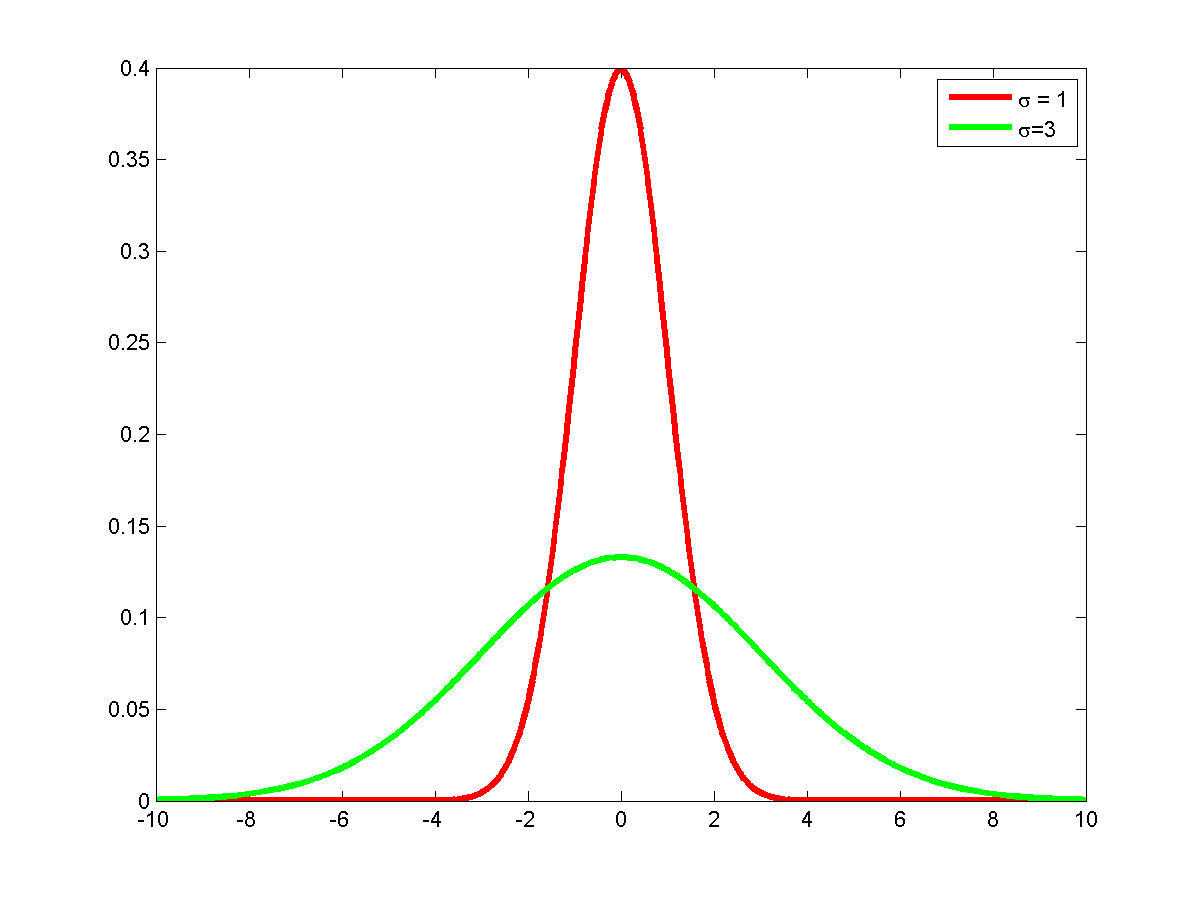
\includegraphics[width=\textwidth]{NormalPlots.png}
\end{figure}

\item For $\mu=2,\, \sigma=0.5$, \medskip \\
Let $F(x)=P(X \le x)= \text{Cumulative Distribution Function},$ we can calculate that:

\begin{enumerate}
\setlength{\itemsep}{.1in}
\renewcommand{\labelenumii}{\roman{enumii}.}

\item $P\{ X \ge 4\} = \int \limits_{4}^{\infty}f_{X}(x)dx=1-F(4)=3.2 \times 10^{-5}.$

\item $P\{  -2 \le X  \le 4 \} = \int \limits_{-2}^{4}f_{X}(x)dx = F(4)-F(-2) = 0.9999.$

\item  $\begin{aligned}[t]P( X \in A) &= \int \limits_{-2}^{4}f_{X}(x)dx+\int \limits_{8}^{100}f_{X}(x)dx \\ &= (F(4)-F(2))+(F(100)-F(8))=0.9999.\end{aligned}$\\[.4cm]
\end{enumerate}

Similarly, for $\mu=2,\, \sigma=5$,
\begin{enumerate}
\setlength{\itemsep}{.1in}
\renewcommand{\labelenumii}{\roman{enumii}.}

\item $P\{ X \ge 4\} = \int \limits_{4}^{\infty}f_{X}(x)dx=1-F(4)=0.3446.$

\item $P\{  -2 \le X  \le 4 \} = \int \limits_{-2}^{4}f_{X}(x)dx = F(4)-F(-2) = 0.4436.$

\item  $\begin{aligned}[t]P( X \in A) &= \int \limits_{-2}^{4}f_{X}(x)dx+\int \limits_{8}^{100}f_{X}(x)dx \\ &= (F(4)-F(2))+(F(100)-F(8))= 0.5586.\end{aligned}$
\end{enumerate}

\item $Y$ is a Gaussian random variable with mean $2\mu + 4$ and variance $4\sigma^2$. \\
\framebox[1.1\width]{$\therefore \mu_Y = 8 ~~ \text{and} ~~ \sigma_Y = 1.$}
\end{enumerate}

\newpage
%Prob. 5  Marginal and Conditional Density
\noindent \textbf{Problem 5:}
\begin{enumerate}
\setlength{\itemsep}{.1in}
\renewcommand{\labelenumi}{(\alph{enumi})}

\item $f_{XY}(x,y)dy$ is a density so we have:
$$\hfill \int \limits_{0}^{1} \big[\int \limits_{0}^{2} f_{XY}(x,y)dy\big]dx=1 \hfill$$
As given, $f_{XY}(x,y)dy=K(x+y)^2$,
$$\begin{aligned}[t] \therefore ~~ 1 &= K \int \limits_{0}^{1} \big[\int \limits_{0}^{2}(x^2+2xy+y^2)dy\big]dx \\ &= K \int \limits_{0}^{1} \big[2x^2+\frac{2x}{2}y^2 \big|_{0}^{2} + \frac{1}{3}y^3\big|_{0}^{2}\big]dx \\
&= K \int \limits_{0}^{1} \big[2x^2+4x + \frac{8}{3} \big]dx \\
&= K \big \{ \big( \frac{2}{3}x^3+2x^2 + \frac{8}{3}x \big) \big|_{0}^{1} \big \}\\
&= K\cdot \frac{16}{3} \hspace{10pt} \Longrightarrow \hspace{10pt}
\boxed{K = \frac{3}{16}}
\end{aligned}$$

\item By definition, the marginal distributions of $X$ and $Y$ are:
$$\hfill \begin{aligned}[t] f_X(x)&=\int \limits_{0}^{2}f_{XY}(x,y)dy=K\int \limits_{0}^{2}(x^2+2xy+y^2)dy\\
&=\frac{3}{16}\big[2x^2+4x+\frac{8}{3}\big]=\frac{3}{8}x^2+\frac{3}{4}x+\frac{1}{2}, \end{aligned} \hfill$$
and $\hfill \begin{aligned}[t]f_Y(y)&=\int \limits_{0}^{1}f_{XY}(x,y)dy=K\int \limits_{0}^{1}(x^2+2xy+y^2)dx\\
&=\frac{3}{16}\big[\frac{1}{3}+y+y^2]=\frac{3}{16}y^2+\frac{3}{16}y+\frac{1}{16}, \end{aligned} \hfill$\\
respectively.\\
\medskip
\\ \underline{\text{Check:}}$$\hfill  \; \begin{aligned}[t] \int_0^1f_X(x)dx &= \frac{1}{8}x^3+\frac{3}{8}x^2+\frac{1}{2}x\big|_0^1=1 \\
\int_0^2 f_Y(y)dy &= \frac{1}{16}\big[ \int_0^2 \big[3y^2+3y+1 \big]dy \big] \\ &= \frac{1}{16}\big[y^3+\frac{3}{2}y^2+y \big]\big|_0^2 = 1\end{aligned} \hfill$$

\item
By definition, the conditional distribution is:
$$\hfill \begin{aligned}[t]f_{X|Y=y}(x)&=\frac{f_{XY}(x,y)}{f_Y(y)}\\&=\frac{\frac{3}{16}(x+y)^2}{\frac{3}{16}(y^2+y+\frac{1}{3})}=\frac{(x+y)^2}{y^2+y+\frac{1}{3}}\end{aligned} \hfill$$
\end{enumerate}
\bigskip
%Prob. 6  Lagrange Multipliers
\noindent \textbf{Problem 6:}
Denote the minimization function as $f$, constraint function as $g$:
$$\hfill \begin{aligned}[t] f(x_1, x_2)&=(x_1)^2+(x_2)^2 \\ g(x_1, x_2)&=x_1+3x_2-4\end{aligned} \hfill$$
\underline{Problem:}
$\hfill \begin{aligned}[t] \min \limits_{(x_1,x_2)\in \real^2}&~~f(x_1,x_2)\\ \text{subject to:} &~~g(x_1,x_2)=0\end{aligned} \hfill$\\
Lagrange function is:
$$\begin{aligned} L(x_1, x_2) &= f(x_1, x_2)+\lambda \; g(x_1,x_2)\\ &=(x_1)^2+(x_2)^2+\lambda(x_1+3x_2-4) \end{aligned}$$
Lagrange multipliers yields a necessary condition for minimization.
\medskip\\
\underline{Necessary Conditions:}
$$\left\{ \begin{aligned} \frac{\partial L}{\partial X}&=\begin{bmatrix} \frac{\partial L}{\partial x_1} \\ \frac{\partial L}{\partial x_2} \end{bmatrix}=\begin{bmatrix}2x_1+\lambda \\ 2x_2+3\lambda \end{bmatrix}=\begin{bmatrix}0 \\ 0 \end{bmatrix}\\ \frac{\partial L}{\partial \lambda}&=x_1+3x_2-4=0 \end{aligned} \right.$$
Solve the equations:
$$\therefore~~x_1=-\frac{1}{2}\lambda,~~x_2=-\frac{3}{2}\lambda.$$

$$\therefore~~\big(-\frac{1}{2}\lambda\big)+3\big(-\frac{3}{2}\lambda\big)-4=0.$$

$$\therefore\boxed{\lambda=-\frac{4}{5}}.$$
So the $(x_1^*,\,x_2^*)$ yields optimal point is:
$$\therefore~~x_1^*=\frac{2}{5}~~ \text{and}~~ x_2^*=\frac{6}{5}.$$

$$\therefore~~(x_1)^2+(x_2)^2=\frac{4}{25}+\frac{36}{25}=\frac{8}{5}.$$

\bigskip
Lagrange multipliers only give us an optimal point, which can be either minimum or maximum. Is this a minimum or a maximum? Maximum is clearly $\infty$! (As shown below)
\begin{figure}[h!]
\centering
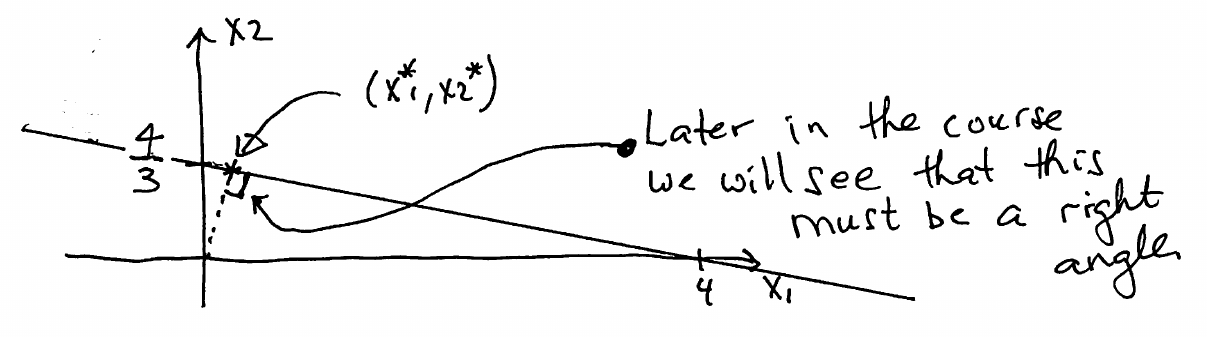
\includegraphics[width=\textwidth]{Prob6Plots.png}
\end{figure}

\newpage

%\bigskip
%Prob. 7  Jointly Gaussian Random Variables
\noindent \textbf{Problem 7:}
From the indicated website
\begin{enumerate}
\setlength{\itemsep}{.1in}
\renewcommand{\labelenumi}{(\alph{enumi})}
\item $X$ and $Y$ each are normally distributed. Moreover,
$$\mu_X=1,\;\sigma_X^2=3;$$
$$\mu_Y=2,\;\sigma_Y^2=2.$$

\item $X$ given $Y=y$ is normally distributed. Moreover,
$$\begin{aligned} \mu_{X|Y} &= \mu_{X}+\frac{\sqrt{5}}{2}(y-\mu_Y) \\ &= 1+\frac{\sqrt{5}}{2}(y-2)=\frac{\sqrt{5}}{2}y+(1-\sqrt{5})\end{aligned}$$
$$\sigma_{X|Y}^{2}=3-\frac{5}{2}=\frac{1}{2}.$$

\item It is $\frac{1}{6}$ of the original variance.

\item Conditional density of $X$ given $Y=10$:
\begin{figure}[h!]
\centering
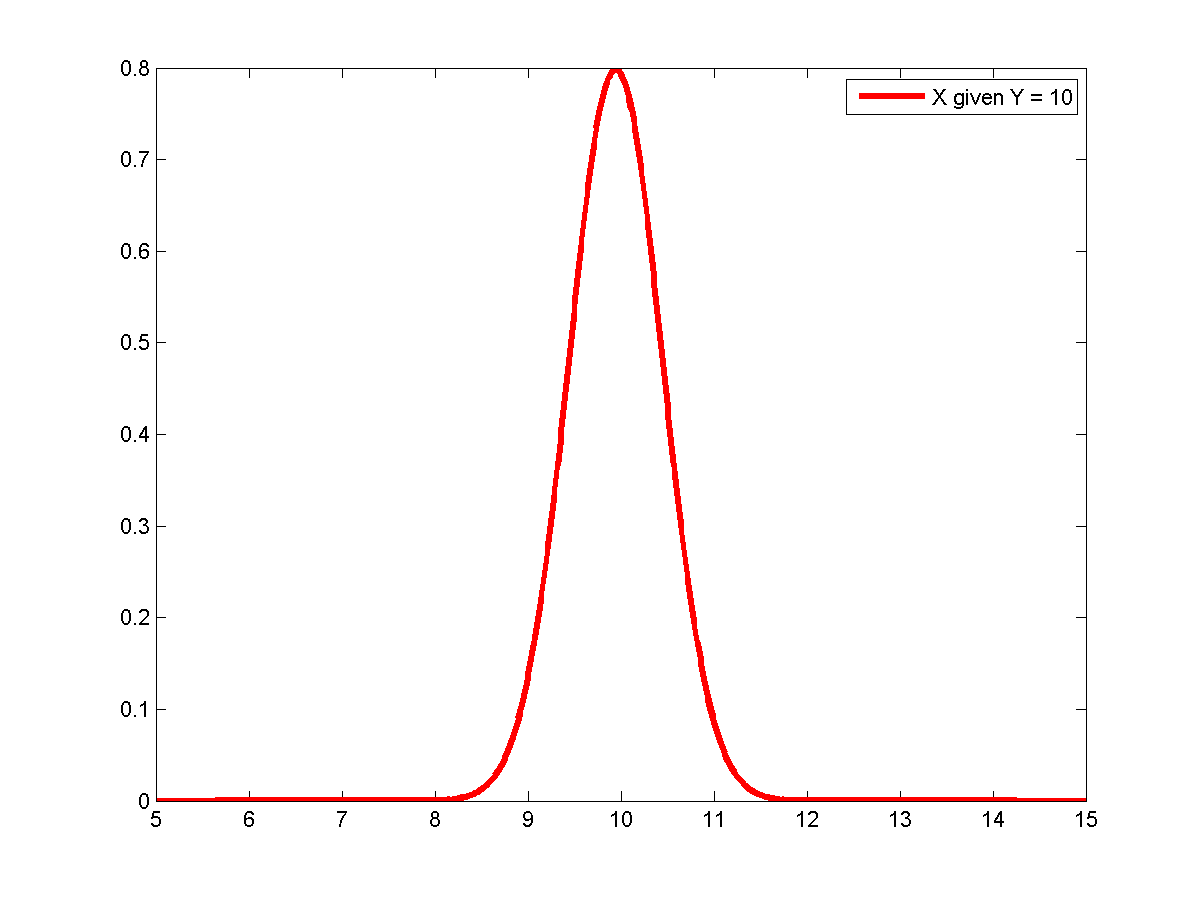
\includegraphics[width=.8\textwidth]{Prob7Plots.eps}
\end{figure}

\end{enumerate}


\end{document}




